
\begin{frame}{Requerimientos de biblioteca de Stack} 
    \begin{itemize}
        \item Protocolo LIFO
        \item El tamano de el stack debe ser configurable por el usuario
    \end{itemize}
\end{frame}

\begin{frame}{Herramientas, googletest} 
    \inputminted[mathescape,
               linenos,
               numbersep=2pt,
               frame=lines,
               bgcolor=White,
               fontsize=\tiny,
               linenos,
               framesep=1mm]{c++}
               {/home/elf/PersonalProjects/UnitTestTalk/src/code/main.cpp} 
\end{frame}

\begin{frame}{Biblioteca Stack, sin tests, todo verde} 
\end{frame}

\begin{frame}{Stack} 
    \begin{itemize}
        \item Comportamiento LIFO.
    \end{itemize}
\end{frame}

\begin{frame}{Incluyendo mi Stack} 
    \inputminted[mathescape,
               linenos,
               numbersep=2pt,
               frame=lines,
               bgcolor=White,
               fontsize=\tiny,
               linenos,
               framesep=1mm]{c++}
               {/home/elf/PersonalProjects/UnitTestTalk/src/code/imports.cpp} 
\end{frame}

\begin{frame}{Primer Acercamiento} 
    \inputminted[mathescape,
               linenos,
               numbersep=2pt,
               frame=lines,
               bgcolor=White,
               fontsize=\tiny,
               linenos,
               framesep=1mm]{c++}
               {/home/elf/PersonalProjects/UnitTestTalk/src/code/testSkeleton.cpp} 
\end{frame}

\begin{frame}{Primer Acercamiento, salida} 
\end{frame}

\begin{frame}{Primer Acercamiento, implementando} 
    \inputminted[mathescape,
               linenos,
               numbersep=2pt,
               frame=lines,
               bgcolor=White,
               fontsize=\tiny,
               linenos,
               framesep=1mm]{c++}
               {/home/elf/PersonalProjects/UnitTestTalk/src/code/stack0.cpp} 
\end{frame}

\begin{frame}{Primer Acercamiento, salida} 
\end{frame}

\begin{frame}{Creando el primer exito} 
    \inputminted[mathescape,
               linenos,
               numbersep=2pt,
               frame=lines,
               bgcolor=White,
               fontsize=\tiny,
               linenos,
               framesep=1mm]{c++}
               {/home/elf/PersonalProjects/UnitTestTalk/src/code/stack1.cpp} 
\end{frame}

\begin{frame}{Creando el primer exito, salida} 
\end{frame}

\begin{frame}{Algo util} 
    \inputminted[mathescape,
               linenos,
               numbersep=2pt,
               frame=lines,
               bgcolor=White,
               fontsize=\tiny,
               linenos,
               framesep=1mm]{c++}
               {/home/elf/PersonalProjects/UnitTestTalk/src/code/test1.cpp} 
\end{frame}

\begin{frame}{Algo util, salida} 
\end{frame}

\begin{frame}{Tomando Forma} 
    \inputminted[mathescape,
               linenos,
               numbersep=2pt,
               frame=lines,
               bgcolor=White,
               fontsize=\tiny,
               linenos,
               framesep=1mm]{c++}
               {/home/elf/PersonalProjects/UnitTestTalk/src/code/stack2.cpp} 
\end{frame}

\begin{frame}{Tomando Forma, salida} 
\end{frame}

\begin{frame}{Biblioteca Stack} 
    \begin{itemize}
        \item Casos bordes
    \end{itemize}
\end{frame}

\begin{frame}{POP de un stack vacio} 
    \inputminted[mathescape,
               linenos,
               numbersep=2pt,
               frame=lines,
               bgcolor=White,
               fontsize=\tiny,
               linenos,
               framesep=1mm]{c++}
               {/home/elf/PersonalProjects/UnitTestTalk/src/code/emptyStackTest.cpp} 
\end{frame}

\begin{frame}{POP de un stack vacio, salida} 
\end{frame}

\begin{frame}{POP de un stack vacio, implementacion} 
    \inputminted[mathescape,
               linenos,
               numbersep=2pt,
               frame=lines,
               bgcolor=White,
               fontsize=\tiny,
               linenos,
               framesep=1mm]{c++}
               {/home/elf/PersonalProjects/UnitTestTalk/src/code/EmptyStackException.cpp} 
\end{frame}

\begin{frame}{POP de un stack vacio, salida} 
\end{frame}

\begin{frame}{POP de un stack vacio, implementacion stack} 
    \inputminted[mathescape,
               linenos,
               numbersep=2pt,
               frame=lines,
               bgcolor=White,
               fontsize=\tiny,
               linenos,
               framesep=1mm]{c++}
               {/home/elf/PersonalProjects/UnitTestTalk/src/code/stack3.cpp} 
\end{frame}

\begin{frame}{POP de un stack vacio, salida} 
\end{frame}

\begin{frame}{Mas casos de borde} 
    \begin{itemize}
        \item Limite de tamano de el stack, tiene que ser configurable por el usuario
    \end{itemize}
\end{frame}

\begin{frame}{Tamano configurable} 
    \inputminted[mathescape,
               linenos,
               numbersep=2pt,
               frame=lines,
               bgcolor=White,
               fontsize=\tiny,
               linenos,
               framesep=1mm]{c++}
               {/home/elf/PersonalProjects/UnitTestTalk/src/code/configurableSizeTest.cpp} 
\end{frame}

\begin{frame}{Tamano configurable, salida} 
\end{frame}

\begin{frame}{Tamano configurable, implementacion} 
    \inputminted[mathescape,
               linenos,
               numbersep=2pt,
               frame=lines,
               bgcolor=White,
               fontsize=\tiny,
               linenos,
               framesep=1mm]{c++}
               {/home/elf/PersonalProjects/UnitTestTalk/src/code/stack4.cpp} 
\end{frame}

\begin{frame}{Tamano configurable, salida} 
\end{frame}

\begin{frame}{Excede limite de tamano} 
    \inputminted[mathescape,
               linenos,
               numbersep=2pt,
               frame=lines,
               bgcolor=White,
               fontsize=\tiny,
               linenos,
               framesep=1mm]{c++}
               {/home/elf/PersonalProjects/UnitTestTalk/src/code/ExceedsStackSizeException.cpp} 
\end{frame}

\begin{frame}{Importo codigo} 
    \inputminted[mathescape,
               linenos,
               numbersep=2pt,
               frame=lines,
               bgcolor=White,
               fontsize=\tiny,
               linenos,
               framesep=1mm]{c++}
               {/home/elf/PersonalProjects/UnitTestTalk/src/code/finalImports.hpp} 
\end{frame}

\begin{frame}{Importo codigo, salida} 
\end{frame}

\begin{frame}{Codigo final} 
    \inputminted[mathescape,
               linenos,
               numbersep=2pt,
               frame=lines,
               bgcolor=White,
               fontsize=\tiny,
               linenos,
               framesep=1mm]{c++}
               {/home/elf/PersonalProjects/UnitTestTalk/src/code/stack5.cpp} 
\end{frame}

\begin{frame}{Codigo final, salida} 
\end{frame}

\begin{frame}{Todos los tests} 
    \inputminted[mathescape,
               linenos,
               numbersep=2pt,
               frame=lines,
               bgcolor=White,
               fontsize=\tiny,
               linenos,
               framesep=1mm]{c++}
               {/home/elf/PersonalProjects/UnitTestTalk/src/code/allTests.cpp} 
\end{frame}

\begin{frame}{Ciclo TDD}
    \begin{center}
        \begin{tikzpicture}[]
            \node[] at (0mm,0mm){
                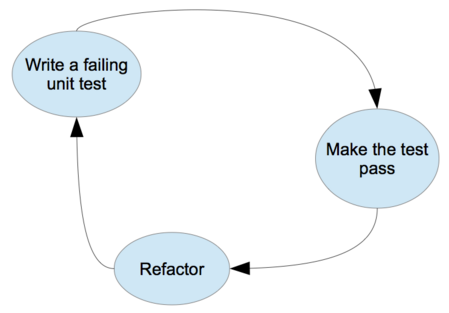
\includegraphics[height=40mm]{/home/elf/PersonalProjects/UnitTestTalk/figures/tddCycle.png}\hspace{5mm}
            };
        \end{tikzpicture}
    \end{center}
\end{frame}

\begin{frame}{Test Driven Development} 
    \begin{itemize}
        \item Rapida y continua retro-alimentacion
        \item TDD abilita refactoring
        \item Lecciones aprendidas, experiencias ganadas no se pierden, quedan en los tests
    \end{itemize}
\end{frame}

\begin{frame}{Test Driven Development} 
    \begin{itemize}
        \item Esto trae consigo desarrollo de software incremental e iterativo
        \item El codigo final generalmente esta bien disenado y 
            \textcolor{red}{tiene tests unitarios!!!!}
        \item No es la respuesta a todos los problemas en desarrollo de software, pero
            definitivamente una mejor al hack, hack, hack and fix
    \end{itemize}
\end{frame}
